\documentclass[12pt,a4paper,oneside,brazil]{abntex2}

% Pacotes que serão utilizados%
\usepackage{lmodern}
\usepackage[utf8]{inputenc}
\usepackage[brazil]{babel}
\usepackage[T1]{fontenc}
\usepackage{indentfirst}
\usepackage{graphicx}
\usepackage{microtype}
\usepackage{wrapfig}
\usepackage[backend = biber, style=abnt]{biblatex}
\addbibresource{Referencias.bib}

% Informações do documento %
\title{Notas Economia Monetária}
\author{Thiago Oliveira Coelho}
\date{\today}
	
\begin{document}
\pagestyle{plain}
\pagenumbering{arabic}
\maketitle
\begin{center}
Resumo baseado em \cite{rossetti98}
\end{center}
\tableofcontents
\chapter{1ª Unidade}

\section{O que é moeda?}
A moeda é tudo que possa exercer as seguintes funções:
\begin{itemize}
\item Função essencial de intermediação de trocas;
\item Serve como medida de valor. As mercadorias tem seu valor mensurado na moeda para simplificação das relações de troca. Sem a moeda a quantidade de relações de troca seria quantificada do seguinte modo: 
\[ RT = \frac{n (n-1)}{2}\]
Sendo:
\begin{itemize}
\item RT: Relações totais de troca;
\item n: Número de mercadorias da economia.
\end{itemize}
\item Servir como reserva de valor.
\end{itemize}
Uma boa moeda também necessita das seguintes características:
\begin{itemize}
	\item Divisibilidade: Possuir múltiplos e submúltiplos;
\item Facilidade de transporte, manuseio e transferabilidade;
\item Indestrutibilidade: Ser resistente.
\end{itemize}

O preço do numerário (equivalente geral) da economia pode ser dado por:
\[P_n = \frac{1}{P}\] 
Aonde:
\begin{itemize}
\item $P_n$: preço do numerário;
\item P: Nível de preços da economia.
\end{itemize}

\section{Lei de Gresham}
A lei de Gresham diz: 
\begin{quote}
"A moeda ruim expulsa a moeda boa de circulação."
\end{quote}
Isso ocorre pois os agentes tenderão a segurar a moeda boa como reserva de valor, tirando esta de circulação.

\section{Histórico da moeda}
A moeda possui várias fases, que não são necessariamente seguidas de forma linear:
\begin{itemize}
\item Moeda mercadoria: Um bem aceito como compensação por grande parte da população pode servir com equivalente geral.
\item Metalismo: Moeda produzida a partir de algum metal.
\item Papel-moeda e Fiduciária: A primeira possui lastro, que pode, ou não, ser integral. Já a fiduciária está lastreada em nada mais que a confiança dos consumidores na própria moeda.
\item Plástica: Cartões de crédito e moeda invisível.
\end{itemize}

\section{Teoria Quantitativa da Moeda}
Existem algumas teorias diferentes:
\begin{itemize}
\item Banking School: $ M = f(P) $
\item Currency School: $ P = f(M) $
\item Fisher: $ M V_t = P T $
\end{itemize}
Aonde:
\begin{itemize}
\item M: Quantidade de moeda;
\item P: Nível de preços;
\item $V_t$: Velocidade das transações;
\item T: Volume físico de transações efetivadas.
\end{itemize}
A equação de fischer é a mais comentada, e ela serve para ilustrar os impactos da quantidade da moeda no nível de preços. Ela irá passar por mudanças devido ao fato de a quantidade transacionada e a velocidade de transações serem de difícíl mensuração. A nova equação de fischer se torna:
\[ M V_r = P Y\] 
Sendo os novos elementos:
\begin{itemize}
\item $ V_r$: Velocidade renda circulação da moeda [Fluxos monetários que contribuem para o PIB]
\item $Y$: Renda
\end{itemize}
Um ponto se manteve com a nova equação: A velocidade é constante no curto prazo. Junto com o pressuposto clássico de que a economia sempre estava no pleno emprego se obtém a dicotomia clássica: O lado real e monetário da economia não interagem.  Porém com essa nova equação é possível obter o vetor de preços absolutos da economia: \newline
Supondo:
\begin{itemize}
\item Sendo o numerário o item n (final) dos vetores:
\item Vetor quantidade: $Q_n  = [Q_1,Q_2, ...., Q_n]$;
\item Vetor preço da mercadoria sobre preço numerário: $\frac{P}{P_n}n =[(\frac{P}{P_n}1), ..., \frac{P_n-1}{P_n}n, 1]$.
\item Dividimos e multiplicamos o vetor resultante (preços nominais) por $P_n$.
\end{itemize}
Podemos obter o vetor preços absolutos:
\[ \frac{(P_1 Q_1, P_2 Q_2,.....)}{P_n}*P_n \Rightarrow M V = \frac{P_1}{P_n} P_n Q+1 + \frac{P_2}{P_n} P_n Q_2  + ..... + P_n Q_n\]

\section{Contribuição de Cambridge}
Se modifica a equação original:
\[MV = PY  \Rightarrow M = \frac{1}{V} P Y \Rightarrow K= \frac{1}{V} \Rightarrow M^d= K P Y\]
Sendo K o coeficiente de retenção da moeda ou tempo médio de retenção da moeda pelos agentes.A evolução quanto a original seria por considerar a demanda por moeda.\\

\section{Contribuição de Friedman e Monetaristas}
Friedman diria que a demanda por moeda seria função:
\[ \frac{M^d}{P} = f(Y^+_p , i^+ , EP^- , w^+ , G)\]
Sendo:
\begin{itemize}
\item $Y_p$: Renda permanente;
\item i: Taxa de juros;
\item EP: Expectativa de inflação;
\item w: Composição da riqueza;
\item G: Preferências.
\end{itemize}
Para se obter a relação entre nível de preços e quantidade de moeda os monetaristas usam:
\begin{large}
\[ P = \frac{M^s}{\frac{M}{P}^d}\]
\end{large}

Conclusões:
\begin{itemize}
\item Há sim relação entre oferta de moeda e nível de preços
\item Nem toda emissão é inflacionária: Se $\triangle M^s = \triangle \frac{M}{P}^d $ então P continua o mesmo.
\item Política monetária seria equivaler a oferta de moeda a sua demanda.
\item Pode haver inflação sem emissão: A demanda cai e a oferta se mantém constante.
\end{itemize}

\section{Versão Keynesiana}
Para Keynes existiam alguns motivos pelos quais os agentes demandariam moeda:
\begin{itemize}
\item Motivo-transação: Moeda para transações correntes, bem similar ao modelo clássico. É função direta da renda.
\item Motivo-precaução: Moeda retida a fim de saldar despesas extraordinárias e incertas. É função direta da renda e da incerteza.
\item Motivo-especulação: Retenção de moeda como ativo financeiro. Neste caso os agentes irão reestruturar suas carteiras de ativos e podem estar esperando, por exemplo, mudanças nas taxas de juros. Keynes percebe que, se os preços de títulos estão altos e a taxa de juros baixa, os agente retém moeda pela expectativa de queda de preços destes títulos. Ocorrendo o contrário, com taxas altas e títulos baratos, havia uma preferência pelos títulos e queda na manutenção de saldos monetários como ativos.
\end{itemize}
A grande diferença de Keynes para os clássicos está justamente no motivo-especulação. Um agente decidiria alocar seu excedente em títulos da seguinte forma: O valor que este estaria disposto a pagar é igual ao rendimento fixo do título dividido pela taxa de juros.
\[ PT = \frac{RT}{i}\]
Keynes irá falar do lado psicológico da taxa de juros: todos teriam uma taxa de juros "normal"($ i_n$) subjetiva obtida a partir das experiências passadas do agente, uma espécie de média ponderada. Quando a taxa de mercado destoasse da taxa normal, esperaríamos uma regressão a média.
Como é possível expressar o juros desta forma: $i = \frac{RT}{PT}$ e os ganhos em termos percentuais desta forma: $ g = \frac{PV^* - PT}{PT}$ aonde $PV^*$ representa o preço de venda do título. Nossa nova euqação de retorno total do título fica:
\[ RTT = i + g\]
Haveria também uma taxa de juros crítica ($i_c$), que seria aquela que igual o rendimento total do título a 0. Essa taxa nos ajuda a definir se o agente possuiria preferência por título ou moeda,. No modelo keynesiano os agentes teriam um portfólio somente com títulos ou moeda, definido da seguinte forma: $ \omega =  f(B,M)$. Portfólio é uma função de títulos ($B$) e moeda para especulação ($M$).
Assim, dependendo das taxas de mercado ($i_m$) teriamos as seguintes situações:
\begin{itemize}
\item $i_m > i_C \rightarrow RTT > 0 \rightarrow B \succ M$
\item $i_m < i_C \rightarrow RTT < 0 \rightarrow B \prec M$
\item $i_m = i_C \rightarrow RTT = 0 \rightarrow B \preceq M$
\end{itemize}
Podemos agora expressar a alocação individual entre moeda especulativa e títulos de um agente representativo (esquerda) e a distribuição de taxas críticas da população (direta):
\begin{figure}[h]
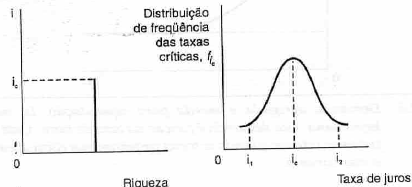
\includegraphics[scale=1]{Decisoes individuais.PNG}
\centering
\caption{Fonte: \cite[p. 77]{rossetti98}}
\end{figure}

Esboçamos agora um gráfico da demanda por moeda:

\begin{figure}
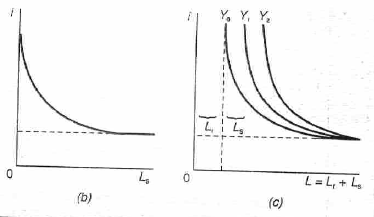
\includegraphics[scale=1]{MD.PNG}
\centering
\caption{Fonte: \cite[p. 79]{rossetti98}}
\end{figure}

Na esquerda a damanda por moeda especulativa e a direita a demanda total por moeda. Note as semelhanças entre a demanda por moeda neste modelo e o gráfico de equilíbrio do mercado financeiro no modelo IS-LM. Demanda agregada total é igual a demanda agregada para transações mais demanda agregada especulativa.
\[ L = L_t(Y) + L_s(i)\]

\section{A contribuição de Tobin}
Tobin apresenta sua \emph{teoria da seleção e composição da carteira de títulos}, na qual tenta se livrar de algumas amarras teóricas que encontra na teoria keynsiana:

\begin{itemize}
\item Taxa de juros e ganhos de capital não são valores constantes, estes apresentam distribuição de probabilidades cujo valor esperado é o ganho mais provável. O risco seria medido pela variância dos resultados esperados: quanto menos concentrada na média (maior desvio padrão) menor a probabilidade do valor assumido ser a média, portanto, maior o risco;
\item Os agentes só estão dispostos a maiores riscos se o retorno total for proporcional a este novo risco.
\item Os agentes possuem uma carteira $W = ( M + B)$, porém não precisam que esta carteira esteja toda em moeda ou títulos. Essa reta W representa uma espécie de restrição orçamentária, mostrando em seus extremos:
\begin{itemize}
\item O ponto em que o risco é minimizado, a carteira é toda composta por moeda e não há retornos decorrentes de juros;
\item O ponto em que o risco é maximizado, a carteira é toda composta por títulos, e o retorno é o máximo possível.
\end{itemize}
\item Os agentes possuem curvas de indiferença que mostram a taxa de substituição entre meoda e títulos pessoal.
\item A maximização dos agentes se dá quando uma das curvas de indiferença tangencia a linha de restrição de alocação da carteira: $max U = f( max RT, min R)$.
\end{itemize}

\begin{wrapfigure}{l}{0.4\textwidth}
	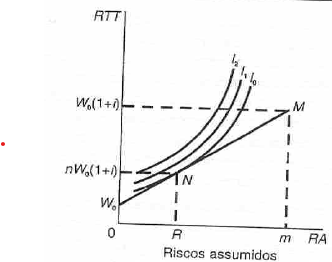
\includegraphics[width=0.4\textwidth]{Contribuicao de Tobin.png}
	\centering
	\caption{Fonte: \cite[p. 82]{rossetti98}}
	
\end{wrapfigure}
Aonde:
\begin{itemize}
\item $RTT$: Retorno Total;
\item $N$: Carteira ótima;
\item $M$: Ponto de risco máximo;
\item $W_0$: Ponto de risco mínimo
\end{itemize}
\clearpage
O retorno deste agente será dado por: 
\[ n W ( 1 + i) \]
Sendo n a fração da carteira aplicada em títulos. Assim, a demanda por moeda especulativa fica subentendida como:
\[ M^{D}_{E} = 1- n \]

\section{Baumol e a demanda por moeda para transações}
A hipótese inspiradora do modelo de Baumol é a de que o saldo de moeda corrente funciona como um estoque na administração. Os agentes teriam uma renda $w$ e durante um período $t$ tentariam manter o mínimo de estoque (saldo monetário em mãos) possível, para assim deixar o resto da renda em títulos e maximizar seu lucro. A cada subdivisão de t, chamada de $n$ o agente saca seu dinheiro (sempre a mesma quantidade), pagando um custo de corretagem $C$ e deixando de ganhar taxa de juros $i$ por aquele dinheiro sacado. Assim, dependendo de quantas vezes fosse necessário sacar dentro deste período t, o agente teria quantidades diferentes de moeda em mãos. Tendo desde um período t completo até este dividido em cinco partes iguais, o agente terá a seguinte porcentagem de moeda em mãos:
\begin{wrapfigure}{l}{0.4\textwidth}
	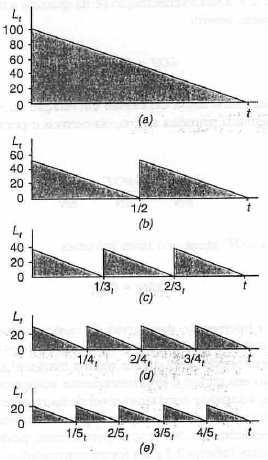
\includegraphics[width=0.4\textwidth]{Baumol.png}
	\centering
	\caption{Fonte: \cite[p. 89]{rossetti98}}
	
\end{wrapfigure}
\newline \newline

Sendo n o número de lotes:
\begin{enumerate}
\item $LT = RT - CT = 0$
\item $LT = \frac{W}{2} \frac{i}{2} - C$
\item $LT = \frac{2 W}{3} \frac{i}{3} - 2C$
\item $LT = \frac{3 W}{4} \frac{i}{4} - 3C$
\item $LT = \frac{4 W}{5} \frac{i}{5} - 4C$
\end{enumerate}

Com esse modelo podemos chegar as seguintes conclusões:
\begin{itemize}
\item A receita total aumenta com o número de transações $n$;
\item A receita marginal decresce a cada transação adicional;
\item A quantidade de moeda retida diminui com aumento do número de transações;
\item Como o agente é maximizador, o número de transações ótimo é aquele no qual $Cmg = Rmg$
\item Mantidos os custos de corretagem, um aumento na taxa de juros implica aumento da receita marginal e consequentemente aumento no número de transações ótimo.
\end{itemize}
Podemos então perceber que \emph{O juros impacta não só a demanda por moeda especulativa, mas também a moeda para fins de transação}. Então demanda por moeda para Baumol é:
\[ M^d = f(Y^+ , i^-) \]
Possíveis críticas ao modelo:
\begin{itemize}
\item Fluxo de pagamentos ser constante e a entrada de renda ser única;
\item Custos de corretagem constantes;
\item Limitado a explicar somente demanda por moeda para transações;
\item Falta de dinâmica;
\item Puramente individual: difíci explicar agregados com o modelo.
\end{itemize}

\section{A base monetária}
Diferenciamos aqui a moeda (que possui liquidez integral) da quase-moeda (alta liquidez). \newline
Desmonetização: Transformação de moeda em quase-moeda (típico de situações de alta inflação). \newline
Agregados monetários (brasileiros):
\begin{itemize}
\item M1: Moeda em poder do público [PmP] + depósitos a vista [DV];
\item M2: M1 + depósitos para investimento + depósitos para poupança + títulos privados;
\item M3: M2 + cotas de fundos + operações compromissadas para títulos federais;
\item M4: M3 + títulos públicos.
\end{itemize}
Em se tratando de M1 temos que Papel moeda em circulação é:
\[ Pmc = PmP + C\]
Sendo $C$ o saldo em caixa dos bancos, já que estes tem de ter uma reserva ($R$) equivalente a taxa compulsória ($\alpha = \frac{R}{DV}$) vezes os depósitos a vista, além de um dinheiro extra  para caso de corrida bancária em caixa. Esta taxa compulsória é definida pelo banco central e faz parte de sua política monetária. Os bancos possuem a capacidade de criar depósitos além daqueles originalmente pertencentes a seus passivos, por isso possuem um multiplicador monetário, que expressa a capacidade deles de criar moeda, neste caso moeda escritural. Este multiplicador é dado por:
\[  m = \frac{DV}{R} \rightarrow m = \frac{1}{\alpha} \]

\subsection{Reservas livres}
As reservas que o banco mantém além daquelas pedidas pelo banco central (compulsórias) são chamadas de reservas livres:
\[ C = \beta DV \]
Sendo $\beta$ o coeficiente que determina a porcentagem de depósitovs a vista que serão revertidos para reservas livres. Nosso multiplicador bancáriose torn então:
\[  m = \frac{1}{\alpha + \beta} \]

\subsection{Multiplicador monetário}
Representa a capacidade de criação de meios de pagamento a partir de moeda primária por meio da economia como um todo.
\[ m_{mon} = \frac{M1}{B} \]
Apesar de representarem coisas diferentes, tanto o multiplicador bancário quanto o monetário são influenciados pelas mesmas coisas:
\begin{itemize}
\item $m$ é função das decisões do banco central e das decisões dos gerentes;
\item $m_{mon}$ é função das decisões do banco central, das decisões dos gerentes e das preferências dos correntistas.
\end{itemize}
A base monetária se configura então como:
\[ B = Pmc + R \rightarrow B = Pmp + C + R \]

\section{Funções do Banco Central}
\begin{enumerate}
\item Executor de política monetária;
\item Agente regulador de bancos comerciais:
\begin{itemize}
\item Realiza intervenções e liquida bancos;
\item É emprestador de última instância;
\end{itemize}
\item Depositário de reservas estrangeiras;
\item Realiza operações com títulos públicos, faz empréstimos e recebe dinheiro do governo federal.
\end{enumerate}
É possível obter a base monetária a partir do balanço do Banco Central: $B$ = Ativo - Passivo não monetário. Podemos fazer um balanço estilizado agregado do mercado financeiro (banco central mais bancos comerciais) da seguinte forma:

\begin{table}[h]
\centering
\begin{tabular}{|l|l|}
\hline
Ativo                   & Passivo              \\ \hline
Reservas internacionais & PmP*                 \\ \hline
Empréstimos ao tesouro  & DV*                  \\ \hline
Títulos federais        & Depósitos do tesouro \\ \hline
Empréstimos             & Depósitos a prazo    \\ \hline
Demais contas do BCB    & Demais contas do BCB \\ \hline
Demais contas dos BC    & Demais contas dos BC \\ \hline
Total do Ativo          & Total do Passivo     \\ \hline
\end{tabular}
\end{table}

Note que PmP e DV formam M1.
\subsection{Instrumentos de política monetária}
\begin{enumerate}
\item Emissão de moeda;
\item Alterar compulsório: $(\alpha)$ alterará o multiplicador $\Rightarrow m = \frac{1}{\alpha + \beta}$
\item Alterar custo de redesconto: irá alterar o comportamento dos bancos comerciais quanto a suas reservas livres $(\beta)$ isto também altera o multiplicador.
\item Operações de mercado aberto : Compra e venda de títulos:
\begin{itemize}
\item O banco central não consegue controlar a liquidez e os juros da economia ao mesmo tempo, ou seja, \emph{há um trade-off entre juros e liquidez};
\item A compra de títulos insere dinheiro na economia, diminuindo a quantidade de moeda em mãos do banco central. A venda de títulos faz o contrário;
\item Essas operações são leilões, nos quais o banco central aceita as propostas de acordo com sua necessidade de política.
\end{itemize}
\item Persuasão: O Banco Central pode utilizar de sua posição como entidade suprema monetária para convencer os bancos comerciais a tomarem certas medidas, como aumentar ou diminuir o número de empréstimos concedidos.
\end{enumerate}

\chapter{2ª Unidade}
A 
\printbibliography
\end{document}
